%Figure~\ref{figure:pipeline} depicts the summarized pipeline of the proposed method. This pipeline contains two main steps: first, the application of 1D-to-2D signal projections, where the 1D signal is transformed into a 2D image, and, then, the application of a \gls{CVC} algorithm to classify the quality of signal into reliable/not-reliable. The 1D-to-2D projection can be performed by using \gls{mtf}, \gls{rp}, or \gls{gaf} algorithms. 


%Moreover, the image aggregation of those three methods, \acrfull{PM}, was used in the scope of this work. It assigns the beforementioned projection methods images to each of the RGB channels. To the best of our knowledge, no previous work has considered a \gls{PM} yet.



%The signal projection approach can produce competitive results with state of art approaches, as using \acrshort{gaf} in combination with Vision Transformer \acrshort{ml} model \cite{1d-to-2d-freitas}. Thereby, they must be described in the following sections, starting with the latest mentioned.


%\begin{figure*}[t!]
%    \centering
%    \includegraphics[width=\linewidth]{imgs/pipeline4.png}
%    \caption{ Proposed pipeline for \acrshort{SQA} using 1D-to-2D projections in combination with \acrshort{CVC}.}
%    \label{figure:pipeline}
%\end{figure*}



% \subsection{Projection Mixture}

% Also, the aforementioned 3 projection methods were combined by image aggregation, feeding the neural networks with an image of 3 channels (usually bijective to the RGB attributes), where each channel is a projection obtained from the same signal.

%The motivation of \gls{rp} usage to project 1D signal into a \gls{2D} space by embedding procedures is to identify time recurrences (correlations) that are not easily apparent in the \gls{1D} signals. These recurrences encode physiological states that can be assessed by searching repeated patterns in the produced 2D images. Similarly, \gls{mtf} can be employed to produce such representation, but by using a Markov chain of first order. Finally, the same end can be achieved using \gls{gaf}, which represents a time series in a polar coordinate system and then it builds a Gramian matrix where each element is the trigonometric sum between different time intervals. In the Gramian matrix, each element is, actually, the cosine of the summation of angles. These algorithms are suitable for characterizing signal quality because the images generated from them produce texture patterns highly correlated with the original waveform of the 1D signal. From Figure~\ref{fig:signals_and_maps}, we can notice that a noisy signal, customarily associated with ‘unreliable’ \gls{SQI}, often presents visual patterns with lower redundancies and higher entropy. On the other hand, reliable signals usually produce projections (or `encoding maps') with lower entropy and harmonious texture patterns.

%% OBSERVATION
%% Podemos omitir para o WCOMP, mas pode detalhar ainda mais na sua dissertação!
%\subsection{Gramian Angular Field}

% The main idea behind \acrfull{gaf} projection method is utilizing the polar coordinate system $ [0,\pi] \times \mathbb{R} $, to represent the signal in a way that the overall shape of the signal curve changes as time passes, since the arc of the circumference increases as the radius increases. Therefore, not mattering if the signal is periodical, its shape changes as time passes. 

% To map a linear signal to such a coordinate system, the following identities were applied to obtain the radius $r_i$ and the angle $\phi_i$ of the $i$-th sample of the signal: ${\phi_i = arccos(x_i)}$, with ${x_i \in \mathbb{R}}, {-1 \leq x_i \leq +1}$; and ${r_i = t_i/N, t_i \in \mathbb{N}}$, with ${N \in \mathbb{R}}$, where $N$ can be used to stretch or to detract the signal along the radius axis. Notice that the signal needs to be rescaled to the interval $[-1,+1]$. 

% However, the signal is yet one-dimensional. Hence, an aggregate operation $Agg$ is applied to each pair to produce the matrix $ GAF = \{Agg(\phi_i,\phi_j)\}_{i,j}$. Examples of those aggregate functions are the $cos(\phi_i + \phi_j)$ function, which produces the Gramian Summation Angular Field ($GAF_S$), and the function $sin(\phi_i - \phi_j)$, that produces the Gramian Difference Angular Field ($GAF_D$). They can be simplified by the use of trigonometric properties, as seen in the following equations:
% \begin{align}
%     GAF_S & = (\vec{x}^T \cdot \vec{x}) - ((\Delta(\vec{x}))^T \cdot \Delta(\vec{x})) = 
%     \cos^{-1}\left( \frac{T_{ij}}{\sqrt{T_{ii} \cdot T_{jj}}} \right) \\
%     GAF_D & = ((\Delta(\vec{x}))^T \cdot \vec{x}) - (\vec{x}^T \cdot \Delta(\vec{x})) = 
%     \sin^{-1}\left( \frac{T_{ij}}{\sqrt{T_{ii} \cdot T_{jj}}} \right)
% \end{align}
% Where $\Delta(\vec{v})$ applies the function $f(x)=\sqrt{1-x^2}$ to $\vec{v}$ element-wise. 

% \subsection{Markov Transition Field}

% The Markov Transition Field's first step is elaborating a Markov chain of first order, considering as states quantile bins containing samples of the signal and defining as a transition of states $S_i \rightarrow S_j$ as the probability of, given the set of all pairs $(x_u,x_{u+1})$ of subsequent signal samples for all $x_u \in q_i$, the subsequent sample $x_{u+i}$ belong to the quantile $q_j$. Then, the Markov chain can be described as the matrix ${M = \{P(S^\prime \rightarrow S_j|S^\prime=S_i)\}_{i,j}}$, where $S^\prime$ is the current state of the Markov chain state machine. Notice that $\sum_j P(S^\prime \rightarrow S_j|S^\prime=S_i) = 1$ for each state $S_i$.

% Nonetheless, the matrix $M$ doesn't fully retain the time sequentiality, since quantiles are sets obtained by value, not by timestamp. For that reason, a second step is made, building a matrix corresponding to the Markov Transition Field, defined as follows:
% \begin{equation}
%     MTF = \{M_{u,v} | x_i \in q_u, x_j \in q_v\}_{i,j}
% \end{equation}
% Where $M_{u,v}$ is the element of the matrix M on the given row and column.

% \subsection{Recurrence Plot}

% Finally, the last method is described, beginning with the transformation of the original signal $\vec{x}_{1 \times n}$ into a matrix $X_{d \times m}$, with $m=n-(d-1)$, where each of the $m$ columns corresponds to a vector $\vec{v}_j$ of $d$ dimensions, such that $\vec{v}_j=[x_j,x_{j+\tau},...,x_{j+\tau \cdot (d-1)}]$, that is, $\vec{v}_j$ is a sequence of $d$ samples of $\vec{x}$, beginning in the position $j$, with time delays of value $\tau$ between them. From that point of view, the matrix $X_{d \times m}$ can be seen as a vector $\vec{X}_m$ with elements of $d$ dimension.

% In the end, each distance between vectors contained in $\vec{X}$ can be compared, leading to the following matrix:
% \begin{equation}
%     RP = \{ D(\vec{X}_i, \vec{X}_j)  \}_{i,j}
% \end{equation}
% Where $D(\vec{X}_i, \vec{X}_j) = || \vec{X}_i - \vec{X}_j ||$. Optionally, it's possible to apply a threshold function $\Theta$ to classify the obtained distances, resulting in the matrix $RP = \{ \Theta(D(\vec{X}_i, \vec{X}_j))  \}_{i,j}$.

\section{Photopletysmograph signal}



\section{Projection Methods}

This section provides an analysis of the projections methods that this thesis used to convert the one-dimensional \gls{PPG} signal into a 2D representation. For example purposes, we will use the signal in figure \ref{fig:methodology:signal}.

\begin{figure}[h]
	\centering
	\adjustbox{height=0.3\textheight}{
		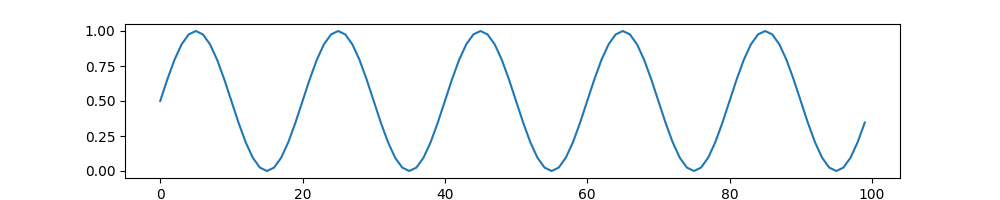
\includegraphics{img/methodology/signal.png}
	}
	\label{fig:methodology:signal}
	\caption{The example signal, with function $f(t)=\sin(\frac{15 \pi t}{500}) + \frac{t}{500}$. }
\end{figure}


\subsection{Recurrence Plot}

The work of Eckmann et al. \cite{rp-1}, of 1987, introduced the \gls{RP} method as a tool for representing visually usefull properties and behaviours of a time series. Since then, its application expanded to various domains, ranging areas such as earth sciences, finances, engineering, chemistry and physics \cite{rp-2}. It also is applicable in life sciences, with attemps on identifying the presence of Parkinson's disease \cite{rp-3}, epileptic seizure \cite{rp-4}, fetal hypoxia \cite{rp-5}, and Alzheimer's disease \cite{rp-6}. Particularly, considering this thesis scope, we can employ \gls{RP} in tasks involving cardiological signal processing, such as cardiac arrythmia classification \cite{rp-7}. Thus, it is likely that this method is usefull in the \gls{SQA} of cardiological signals.  

The \gls{RP}, in essence, represents the ocurrence of recurrences between the phase space values of time instant pairs. For this end, the first step is to embed the time series $X=x_1,x_2,...,x_n \in \mathbb{R}^n$ with $n \in \mathbb{N}$ samples into a phase space, creating a new time series $S=\vec{s_1},\vec{s_2},...,\vec{s_m} \in \mathbb{R}^m \times \mathbb{R}^d$ with $m \in \mathbb{N}$ elements. We can employ the time delays method to represent each element $\vec{s_i} \in \mathbb{R}^d$ of this new sequence $S$ as follows:

\begin{equation}
	\vec{s_i} = (x_i, x_{i + \tau}, x_{i + 2\cdot \tau} ..., x_{i + (d-1) \cdot \tau})
\end{equation}   

\noindent where $d \in \mathbb{N}$ is the dimension and $\tau \in \mathbb{N}$ is the time delay of the phase space. Notice that the lenght $m$ of the sequence $S$ depends on both $d$ and $\tau$ by the equation $m = n - (d-1) \cdot \tau$. Also notice that this embedding is optional, since the choice of the dimension $d=1$ results in $S=X$, the original time series. The figure \ref{fig:phase_space} depicts the phase space of the example signal of the figure \ref{fig:methodology:signal}.

\begin{figure}[h!]
    \centering
    \adjustbox{width=\textwidth}{
        \begin{tabular}{cc}
            \includegraphics[height=0.2\textheight]{img/methodology/delay_phase_space.pdf} &
            \includegraphics[height=0.2\textheight]{img/methodology/delay_phase_space_recurrences.pdf} 
        \end{tabular}
    }
    \caption{On the left, we have the signal of the figure \ref{fig:methodology:signal} on the time delay phase space, without temporal information. Its parameters are dimension $d=2$ and delay $\tau=\RPDelay$. On the right, we have almost the same figure, but with the recurrences represented by red lines $\vec{s_i} - \vec{s_j}$ that links the pair of near points that have a distance bellow $\varepsilon=\RPThreshold$. That figure omits the recurrences to the point itself.}
    \label{fig:phase_space}
\end{figure}


Then, the second step is to build a $m \times m$ matrix $RP$ of recurrences where each cell $RP_{i,j} \in \{0,1\}$ represents the presence or the ausence of a recurrence in a pair of points $\vec{s_i},\vec{s_j}$ of the phase space $S$. We can represent this concept by measuring the distance $||\vec{s_i} - \vec{s_j}||$ between the points of the pair and verifying if it is smaller than a threshold $\varepsilon \in \mathbb{R}$ as the following equation:

\begin{equation}
	RP_{i,j} = \mathcal{H}(\varepsilon - ||\vec{s_i} - \vec{s_j}||)
\end{equation}

\noindent where $\mathcal{H}: \mathbb{R} \mapsto \{0,1\}$ is the Heaviside function. Alternativelly, we can produce an unthresholded version $RP'$ by attributing to each cell the points distance:

\begin{equation}
	RP'_{i,j} = ||\vec{s_i} - \vec{s_j}||
\end{equation}  

\noindent The figure \ref{fig:method:rp} exibits both $RP$ and $RP'$ of the example signal.

\begin{figure}[h!]
	\centering
	\begin{tabular}{cc}
		\frame{
\includegraphics[width=0.35\textwidth]{img/methodology/RecurrencePlot.png}} &
		\frame{\includegraphics[width=0.35\textwidth]{img/methodology/RecurrencePlotUnthresholded.png}} 
	\end{tabular}
	\caption[The resulting recurrence plots of the signal in Figure \ref{fig:methodology:signal}.]{The resulting recurrence plots of the signal in Figure \ref{fig:methodology:signal}, in coherence with the phase space of the Figure \ref{fig:phase_space}. On the left, we have the thresholded version, while on the right we have the unthresholded version.}
	\label{fig:method:rp}
\end{figure}


\subsection{Gramian Angular Field}

% falar sobre GAF

The \gls{GAF}, in summary, encodes the signal into angular relationships between pair of points. The first step to do this is to convert the signal $X=x_1,x_2,...,x_n$, with $n$ samples, into a polar coordinate series $P=p_1,p_2,...,p_n$. One manner to do that is to associate the time $t_i$ to the radius $r_i$ and the value $x_i$ to the angle by the inverse of the cosine as follows:

\begin{equation}
	p_i = (r_i, \phi_i),	
	\begin{cases} 
		\phi_i = cos^{-1}(x_i), & -1 \leq x_i \leq 1\\
		r_i = \frac{t_i}{N}, 	& t_i \in \mathbb{N}, N \in \mathbb{R}
	\end{cases}
\end{equation}    

The second step is to 

\begin{align}
	GASF_{i,j} & = cos(\phi_i + \phi_j) \\
		& = cos(\phi_i) \cdot cos(\phi_j) - sin(\phi_i) \cdot sin(\phi_j) \\
		& = x_i \cdot x_j - \sqrt{1 - x_i^2} \cdot \sqrt{1 - x_j^2}
\end{align}

\begin{equation}
	GASF = X^T \cdot X - \sqrt[\circ 2]{\mathds{1}-X^{\circ 2}}^T \cdot \sqrt[\circ 2]{\mathds{1}-X^{\circ 2}}
\end{equation}


\begin{align}
	GADF_{i,j} & = sin(\phi_i - \phi_j) \\
		& = sin(\phi_i) \cdot cos{\phi_j} - cos(\phi_i) \cdot sin(\phi_j) \\
		& = \sqrt{1 - x_i^2} \cdot x_j - x_i \cdot \sqrt{1 - x_j^2} 
\end{align}

\begin{equation}
	GADF = \sqrt[\circ 2]{\mathds{1} - X^{\circ 2}}^T \cdot X - X^T \cdot \sqrt[\circ 2]{\mathds{1} - X^{\circ 2}}
\end{equation}

\subsection{Markov Transition Field}

\begin{equation}
	W_{i,j} = \frac{\sum\limits_{x_k \in Q_i} \begin{cases} 
			0, & x_{k+1} \not\in Q_j \\
			1, & x_{k+1} \in Q_j
		\end{cases}}{|Q_i|}
\end{equation}


\begin{equation}
	MTF_{i,j} = W_{u,v} | x_i \in Q_u, x_j \in Q_j 
\end{equation}

\section{Proposed Method}

This thesis proposed a novel method. The figure \ref{fig:method} depicts the proposition. First, we transformed the signal into four projections using the three beforementioned algorithms: \gls{GAF} (which generated two variants: \gls{GASF} and \gls{GADF}), \gls{MTF}, and \gls{RP}. Then, we aggregated those projections using composition, that is, we assigned each of them to a different channel of a new input layer. Then, that layer feeded the computer vision model, which contained weights pre-trained on the ImageNet dataset. The figure \ref{fig:input_layer} pictures the feeding process to a three-channeled \gls{CV} model, which consisted in performing a point-wise convolution operation. Finally, that model classified the signal into a binary \gls{SQI}, which indicated if the signal was ``Good'' or ``Bad''. 

\begin{figure}[h!]
	\centering
	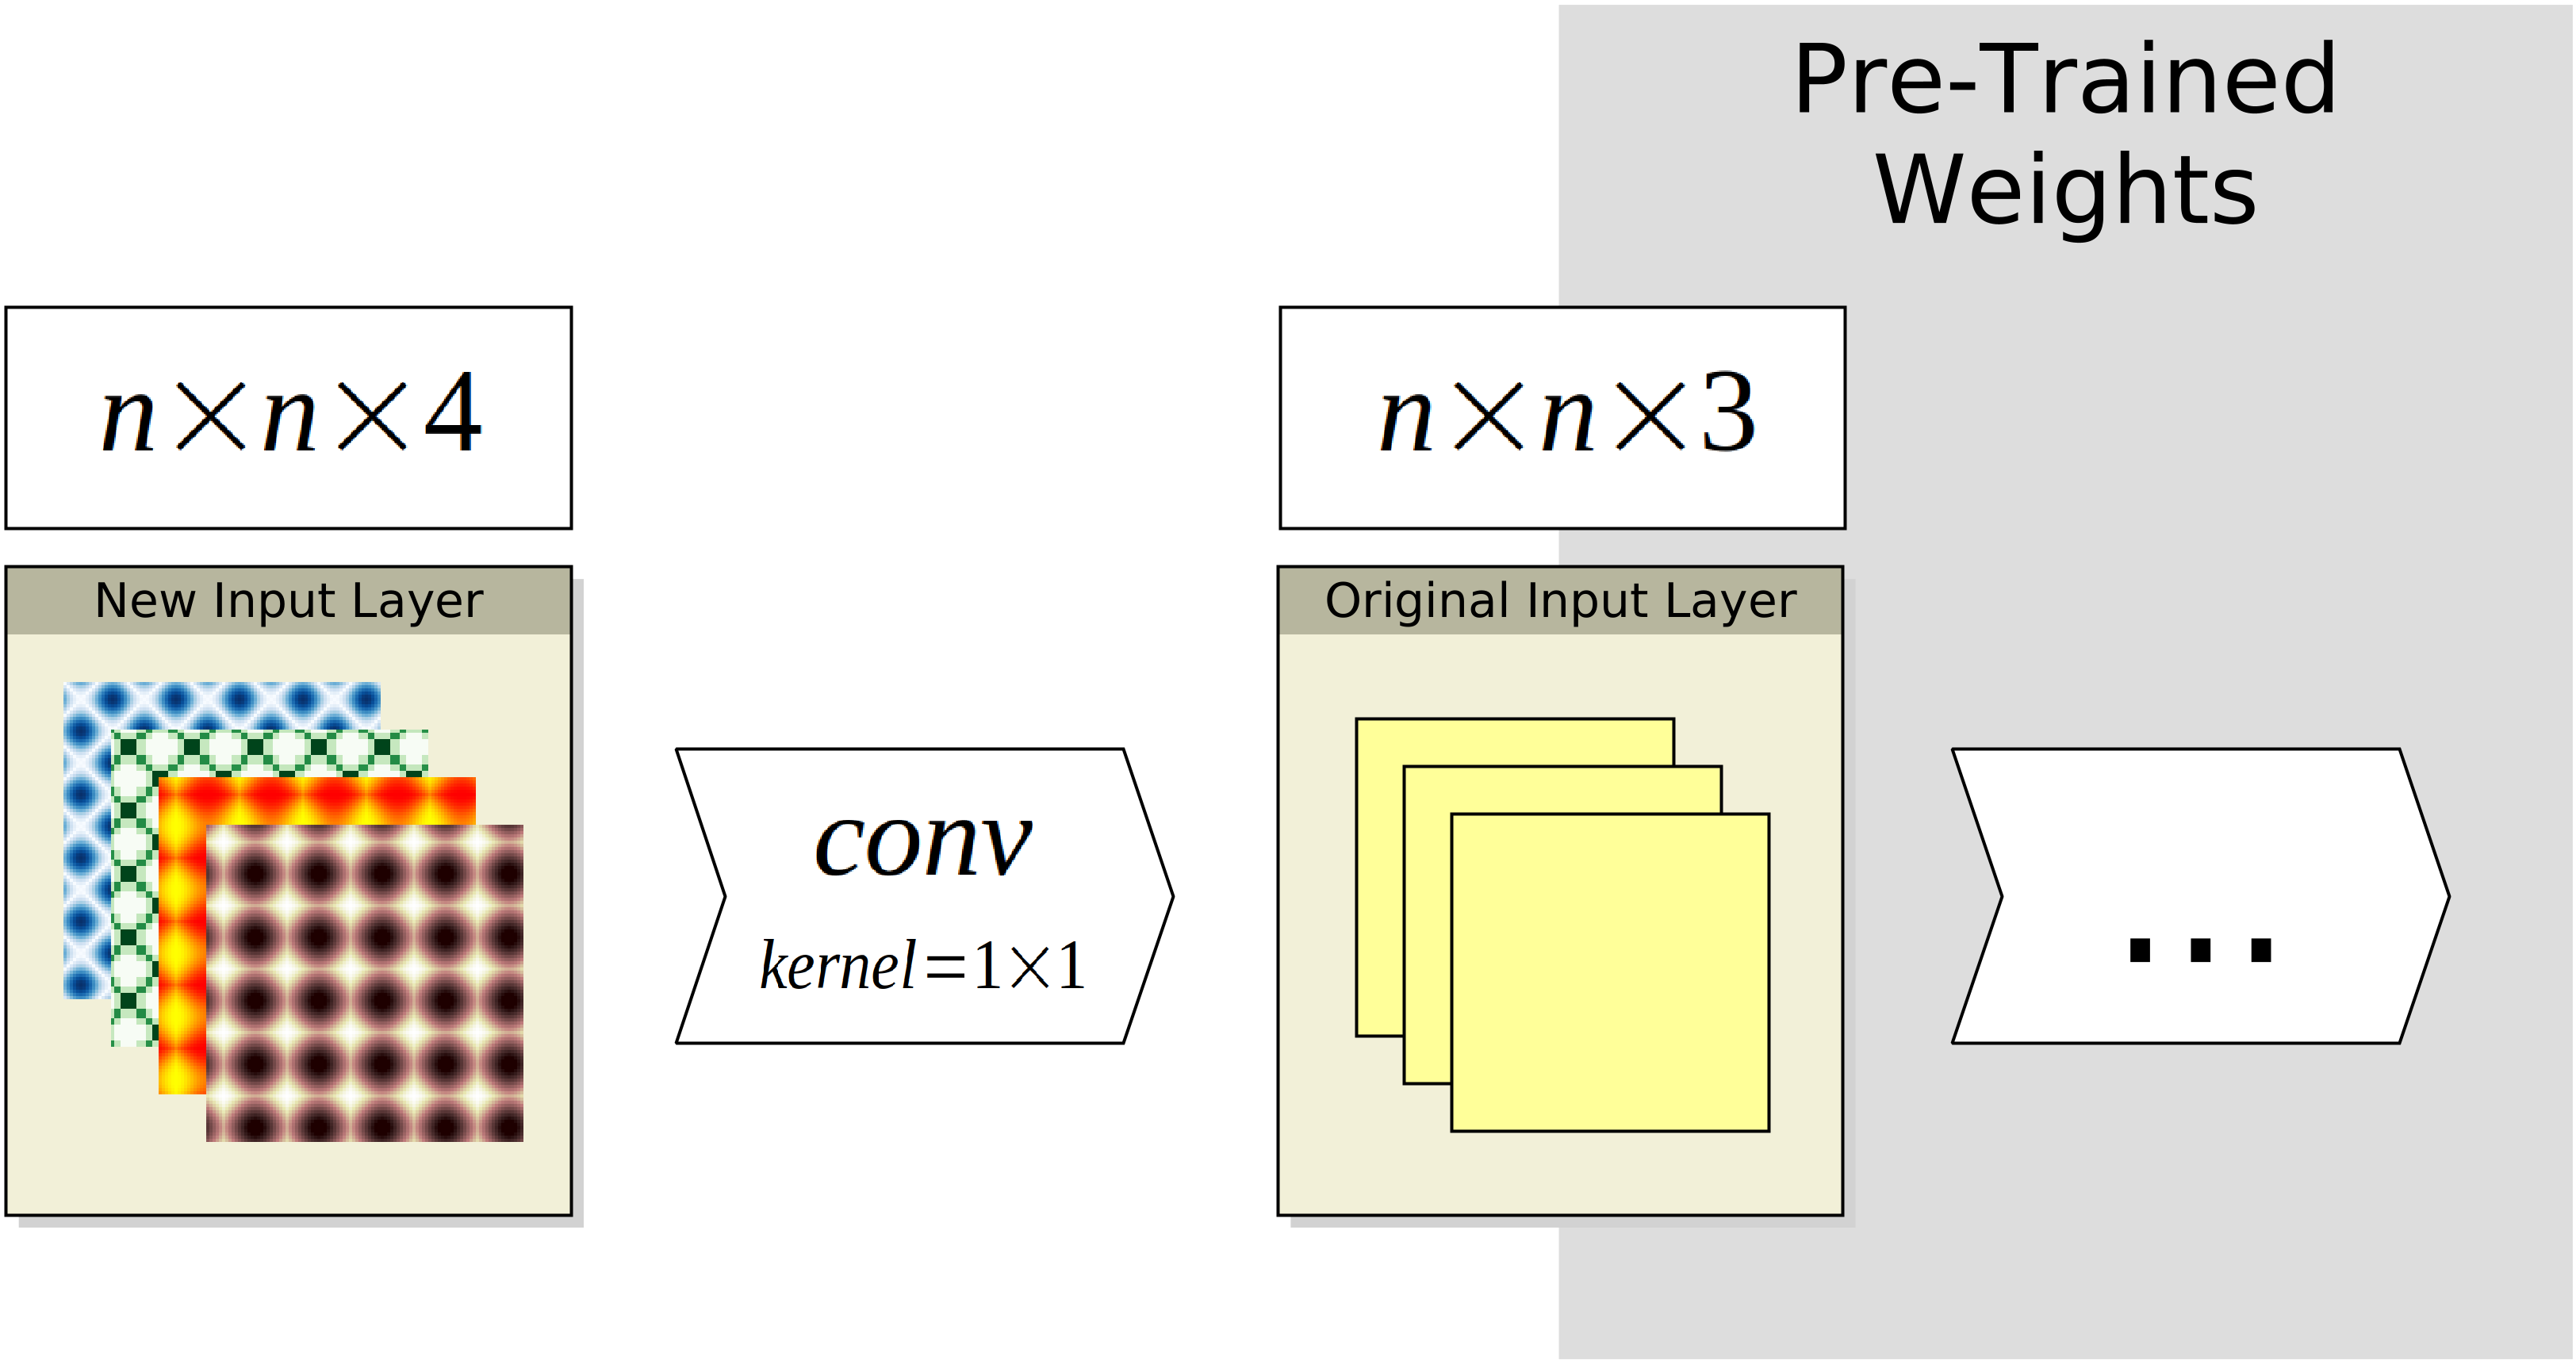
\includegraphics[width=0.8\textwidth]{img/input_layer.png}
	\caption[The three-channeled \acrlong{CV} model feeding process.]{The three-channeled \acrlong{CV} model feeding process. The figure begins in the left, in its input, and progresses to the right. }
	\label{fig:input_layer}
\end{figure}


\begin{figure}[t]
	\centering
	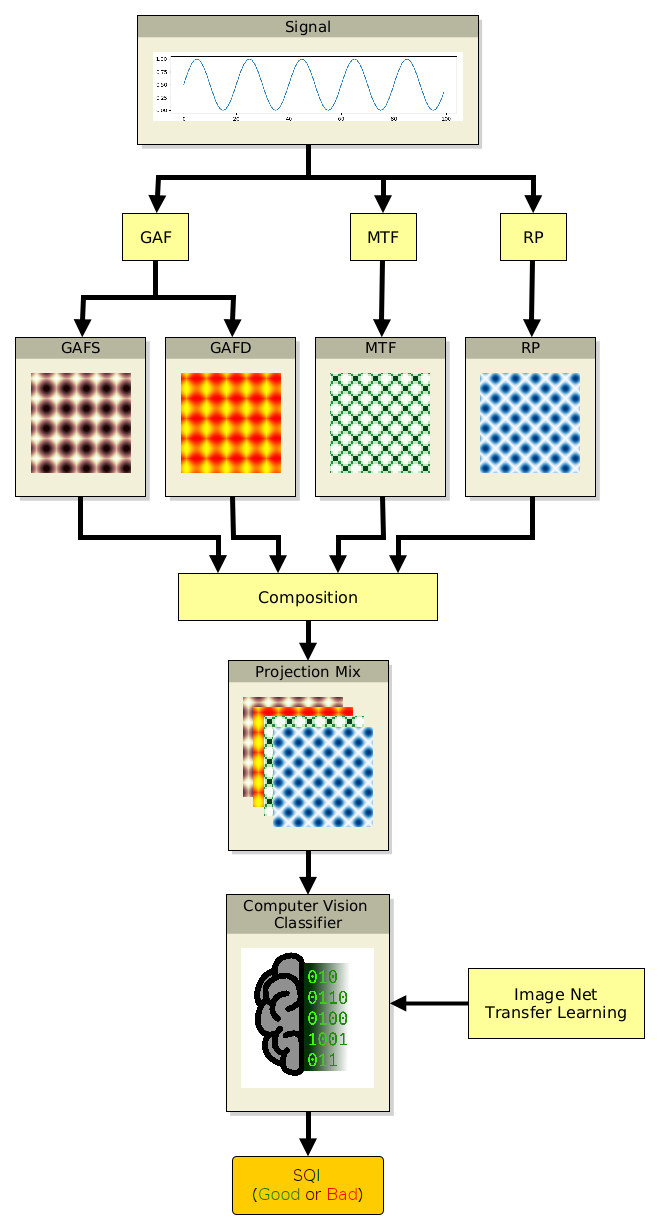
\includegraphics[height=0.95\textheight]{img/method.png}
	\caption{The proposed method. It mainly consisted in feeding the projection composition to the pre-trained \gls{CV} model.}
	\label{fig:method}
\end{figure}


